\documentclass[10pt,conference]{IEEEtran}
\IEEEoverridecommandlockouts
% The preceding line is only needed to identify funding in the first footnote. If that is unneeded, please comment it out.
\usepackage{cite}
\usepackage{amsmath,amssymb,amsfonts}
\usepackage{algorithmic}
\usepackage{graphicx}
\usepackage{textcomp}
\usepackage{xcolor}
\usepackage{capt-of}
\usepackage{hhline}
\usepackage{hyperref}
\hypersetup{
    breaklinks=true,
    colorlinks=true,
    allcolors=blue,
}
\def\UrlBreaks{\do\/\do-}
\urlstyle{same}
\def\BibTeX{{\rm B\kern-.05em{\sc i\kern-.025em b}\kern-.08em
    T\kern-.1667em\lower.7ex\hbox{E}\kern-.125emX}}
\begin{document}

\title{The Impact on Non-Medicaid Expansion on Hospitals in Rural Communities}


\author{\IEEEauthorblockN{Louis Ciotti}
\IEEEauthorblockA{\textit{Data Science} \\
\textit{Utica College}\\
Utica, NY \\
laciotti@utica.edu}
\and
\IEEEauthorblockN{Candyce Griffin}
\IEEEauthorblockA{\textit{Data Science} \\
\textit{Utica College}\\
Utica, NY \\
cagriffi@utica.edu}
\and
\IEEEauthorblockN{Solomon Makoni}
\IEEEauthorblockA{\textit{Data Science} \\
\textit{Utica College}\\
Utica, NY \\
somakoni@utica.edu}
}

\maketitle

\begin{abstract}
U.S. rural communities—from Appalachia and the Deep South to the Midwest and western states to Alaska and Hawaii—share familiar dangers for poor health. These difficulties, including minimal local physicians, poverty, and remote areas, add to the shortage of access to health care. Compared to Urban communities, rural populations have below average median household incomes, an increased amount of children living in poverty, a handful of adults with post-secondary education, higher percentage of uninsured residents below age 65, and increased rates of mortality, according to a 2017 report by the North Carolina Rural Health Research Program(NC RHRP) at The University of North Carolina at Chapel Hill. Rural residents who reside on farms, ranches, reservations, frontiers frequently travel lengthy distances for access to a health care provider. This would involve missing work for their initial appointment or follow-up, causing many to deter or avoid care. Farther distances also cause longer wait times in rural emergency medical services (EMS). That can imperil patients seeking EMS treatment \cite{aamcnews_2017}. The difference in the healthcare needs of rural and urban populations add to the strife of rural healthcare clinics. Rural communities include a greater population of elderly adults, veterans and poor residents than urban areas. These are populations that most often see frequent and complex healthcare needs. Rural areas also have an influx of disease, including the seventh-leading cause of death in the country, diabetes. The healthcare needs of patients can strain rural hospitals that may already be limited to resources \cite{dellasega}.
\end{abstract}

\begin{IEEEkeywords}
Healthcare, Medicare, Hospital Closings, United States, Rural
\end{IEEEkeywords}

\section{Introduction}
According to research from the North Carolina Rural Health Research Program (NC RHRP) of the 27 states that have been reviewed, there has been at least one rural hospital closure since 2010, with the majority of those closures in the South. There has been a total of 17 hospitals closed in Texas since 2010, the most of any state. The state of Tennessee is second with the most closures, with the closing of 10 hospitals since 2010. Georgia comes in 3rd with the 7 total closures. There have been 102 rural hospitals that closed between January 1, 2010, and March 19, 2019, according to NC RHRP, who define a hospital closure as the cessation in the provision of inpatient services \cite{ellison}. There is a characteristic that is most common in these group of states that stands out most---Medicaid has not been expanded. Of the 102 hospital closures in 26 states since 2010, 13 states have refused medicare expansion. Further more as shown in figure \ref{HC_ME}, total closures in states that refused expansion far exceeds those that accepted. Even though there are numerous factors involved in any decision to close a rural hospital, is the fact that many of these states are still refusing federal money that is available for Medicaid expansion. 

\begin{figure*}[htbp]
\centerline{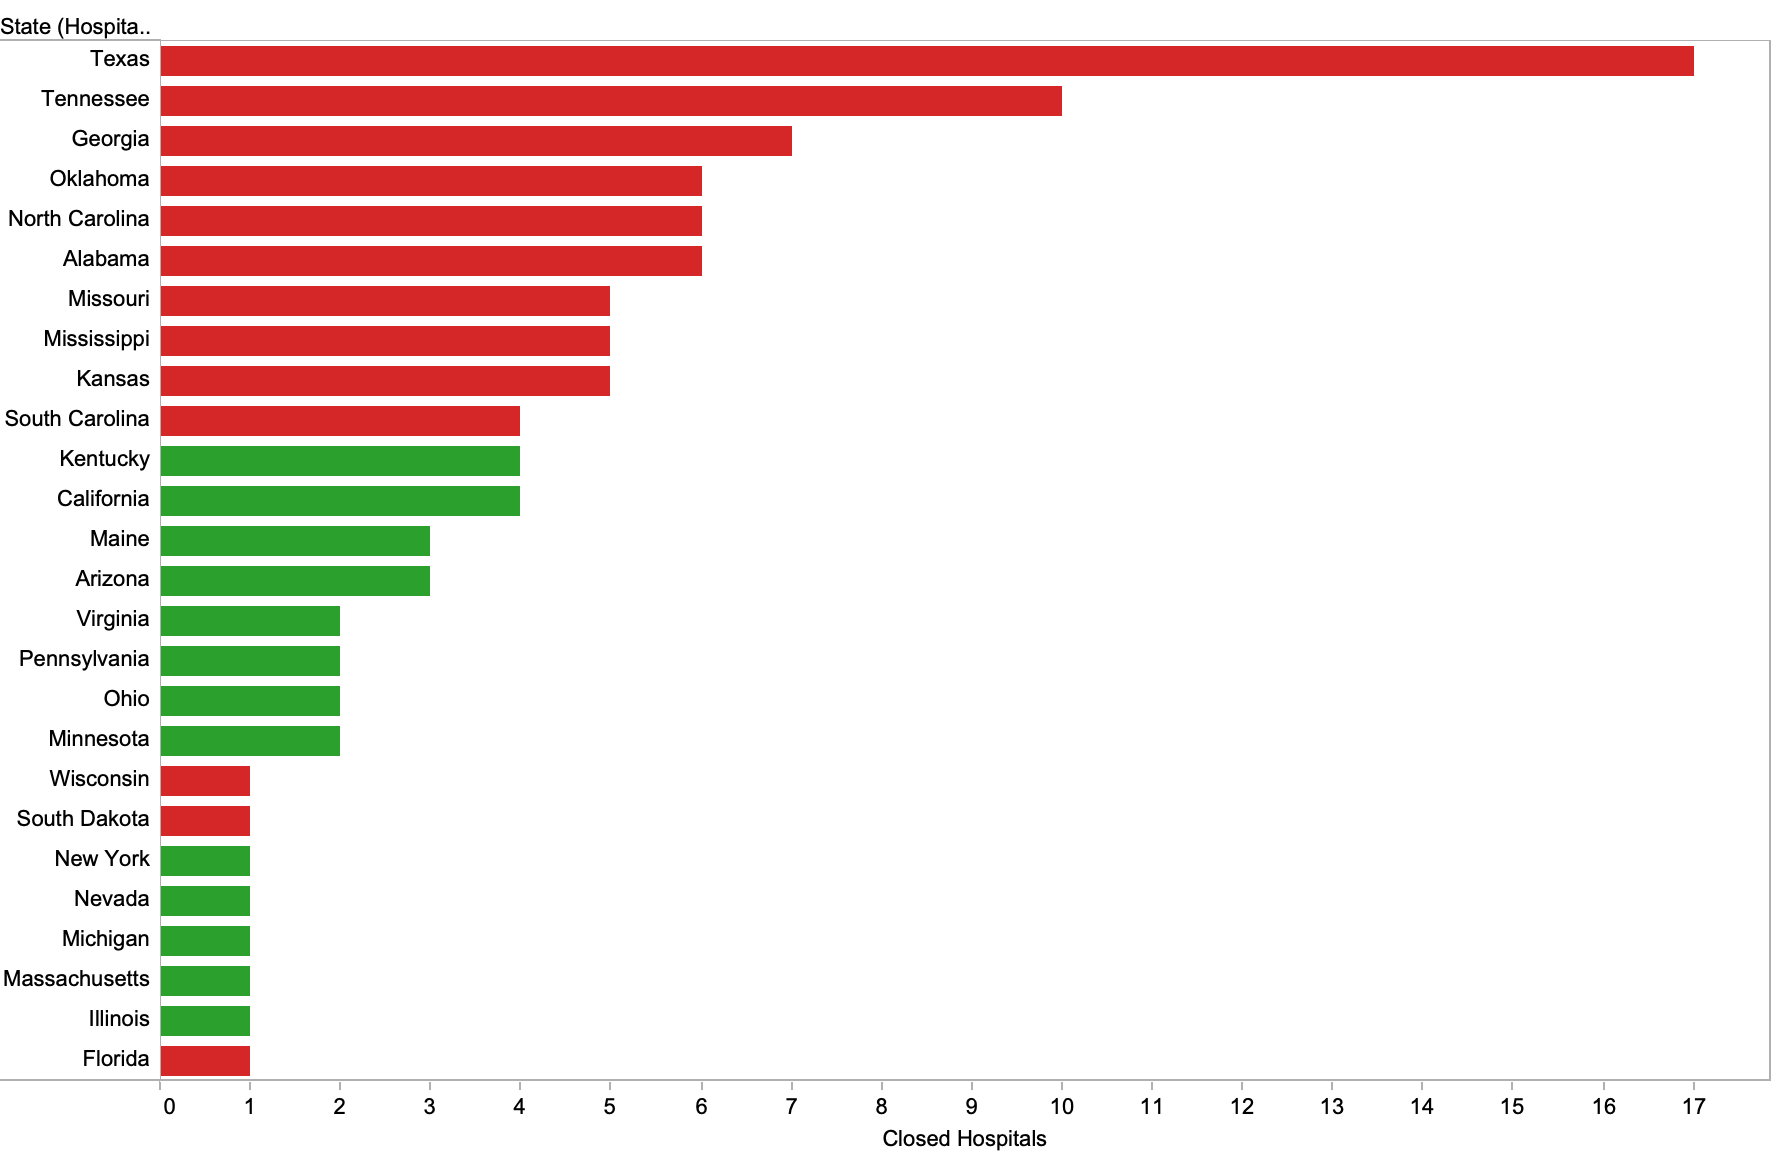
\includegraphics[width=\textwidth]{HC_and_ME.png}}
\caption{Hospital Closures and acceptance of Medicare Expansion\newline \textit{(Red: NO Green: YES)}.}
\label{HC_ME}
\end{figure*}
According to a recent federal report from the US Government Accountability Office on rural hospitals, hospitals in states located in a rural area who increased Medicaid eligibility and enrollment experienced fewer closures. Medicaid expansion was affiliated with improved hospital financial performance and substantially lower likelihoods of closure in rural markets. It is stated in a report on rural health coverage and Medicaid that states that expanded Medicaid witnessed uninsured rates for low-income adults in the rural area decreases three times faster compared to states that did not expand Medicaid. This would indicate in general that when uninsured low-income residents in rural areas and small towns become seriously ill or injured come to their local healthcare facility without insurance coverage have inevitable large bills. Non-expansion states have higher percentages of uninsured residents with no means of paying large bills, whereas expansion states rely on Medicare coverage to close the gap \cite{searing}.

\begin{figure*}[htbp]
\centerline{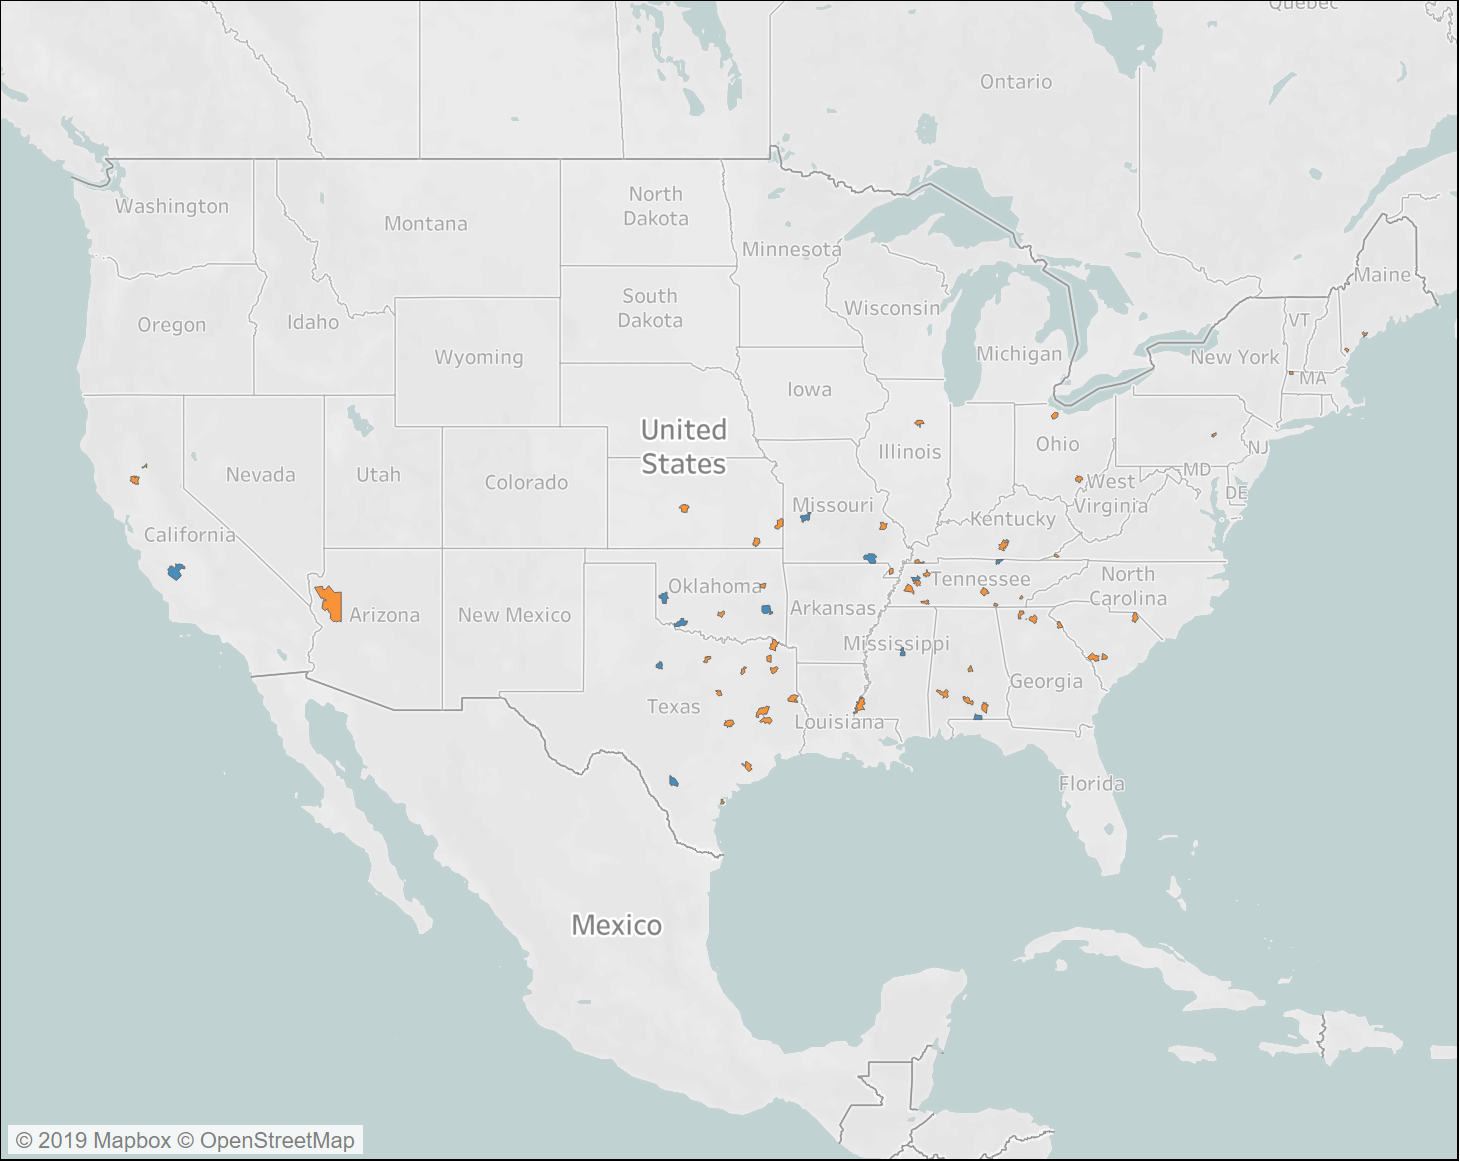
\includegraphics[width=.75\textwidth]{HC_RU.png}}
\caption{Locations of Hospital Closures. (\textit{Blue: Rural Orange: Urban})}
\label{Location_HC}
\end{figure*}

\section{Related Work}
According to the North Carolina Rural Health Research Program, 80 rural emergency clinics have closed since 2010 across 27 states, and in 2016 there were an additional 673 rural medical facilities in danger of closure, according to an iVantage Health Analytics report. The iVantage 2017 Rural Relevance Study also reported that 41 percent of rural healthcare facilities operate at a negative margin. Healthcare facilities in rural communities are struggling to survive. Rural populations, in general, as state above tend include elderly and lower income individuals, healthcare facilities in these communities tend to collect more of their earnings from Medicare and Medicaid reimbursements than facilities within a city. This leaves them progressively powerless against policy changes that impact government reimbursement. The Rural Health Policy project reports that from 2014 to 2015 Medicaid covered 45 percent of children and 16 percent of adults in small towns and rural communities. As a result of this reliance on government funds, any changes to policy or law can intensely influence rural healthcare facilities already in precarious financial positions, so why are they being eliminated at a higher rate without ensuring adequate locations for residents \cite{dellasega}?

\section{Data Description}
At the start of this project, we began with a extensive search of the available data available to the public free at charge, and without usage restrictions. This included several US government agency websites along with sites specific to medicine and public healthcare. As a result of this search were were able to collect the requisite data to investigate how medicaid expansion impacted rural communities. The following data-sets and relevant attributes were used in this project:
\begin{enumerate}
    \item Center for Medicaid Services (2014) Inpatient Prospective Payment System (IPPS) Provider Summary for the Top 100 Diagnosis-Related Groups (DRG). This data set contains a list of hospitals, their addresses including zip codes and states, inpatient payments including Medicare payments. Only the following fields are utilized in this paper:
    \begin{itemize}
        \item Hospitals
        \item Medicare Payments
        \item Zip codes
        \item States
    \end{itemize}
    \item American Communities Survey(ACS) Zip Code Tabulation Area is obtained from census.gov is used to link states population demographics to the hospitals and Medicare payments data. These population numbers are used to paint a picture of the medical needs of states with closing hospitals. The following data attributes are used and derived
    \begin{itemize}
        \item Population
        \begin{enumerate}
            \item High Medical Needs population - Calculated based on percentage of veterans and older population 65 years and above.
            \item Overall population
            \item Rural/Urban Distinction
        \end{enumerate}
    \end{itemize}
    \item Non-Medicare Expansion States as defined in a March 2019 Henry Kaiser Foundation Research. The non-Medicare expansion states are used to associate the policy decisions at the state to the hospital closures.
    \item List of Closed Hospitals since 2010 from the  North Carolina Rural Health Research Program (NC RHRP). This list is an indicator of the size of the problem as each closed hospital implies lack of access for high needs and poor patients. 
\end{enumerate}
    
\section{Methods}
\subsection{Data Collection and Cleansing}
For this paper, we identified the closing hospitals, non-Medicare expansion states, and states that have refusing to accept Medicare under the Affordable Care Act (ACA). The first step after collecting the required data-sets was to open each file an determine how clean the data was along with compatibility with the other data for when we perform the joining step later. Initial data munging was done using excel, particularly to ensure state names were available as two letter abbreviations and that any empty or blank cells would not interfere with the later analysis. Additionally, an excel file was generated to separate the states into 4 regions for analysis and filtering purposes. 
\subsection{Analysis}
Utilizing \emph{Tableau}, the analysis used the software package's built in joining functionalities to combine the ACS provider payments data to Zip Code Tabulation Areas (ZCTA) and to tie geographic demographics data to Medicare payments data. The region excel file was then joined to the data-set to allow additional filtering. With knowledge of Medicare payments, demographics, closures and refusal by states to accept Medicare expansion, the analysis sought to distinguish geographic areas with prevalent hospital closures from the rest of the states. These factors included population sizes, rural/urban distinction, non-Medicare expansion. 
\subsection{Visualization}
The visualization creation process entailed creating geographic maps to indicate distributions of population, Medicare payments, etc. \emph{Tableau} proved to be invaluable in the creating of the geographic maps. Since our data-set contained ZCTA information, the process of simple and the resulting maps provide great insight into out problem statement. Additionally, several bar graphs were developed to to aide in the comparison and to show the compositions of states with closing hospitals as well as their medical needs populations. Ounce again emph{Tableau} was used as the main tool for creating individual visualizations as well dashboards with applicable filters implemented to interact with the visualizations and layers of the data. The resulting dashboard is shown in figre 

\ref{dashboard}.
\begin{figure}[htbp]
\begin{center}
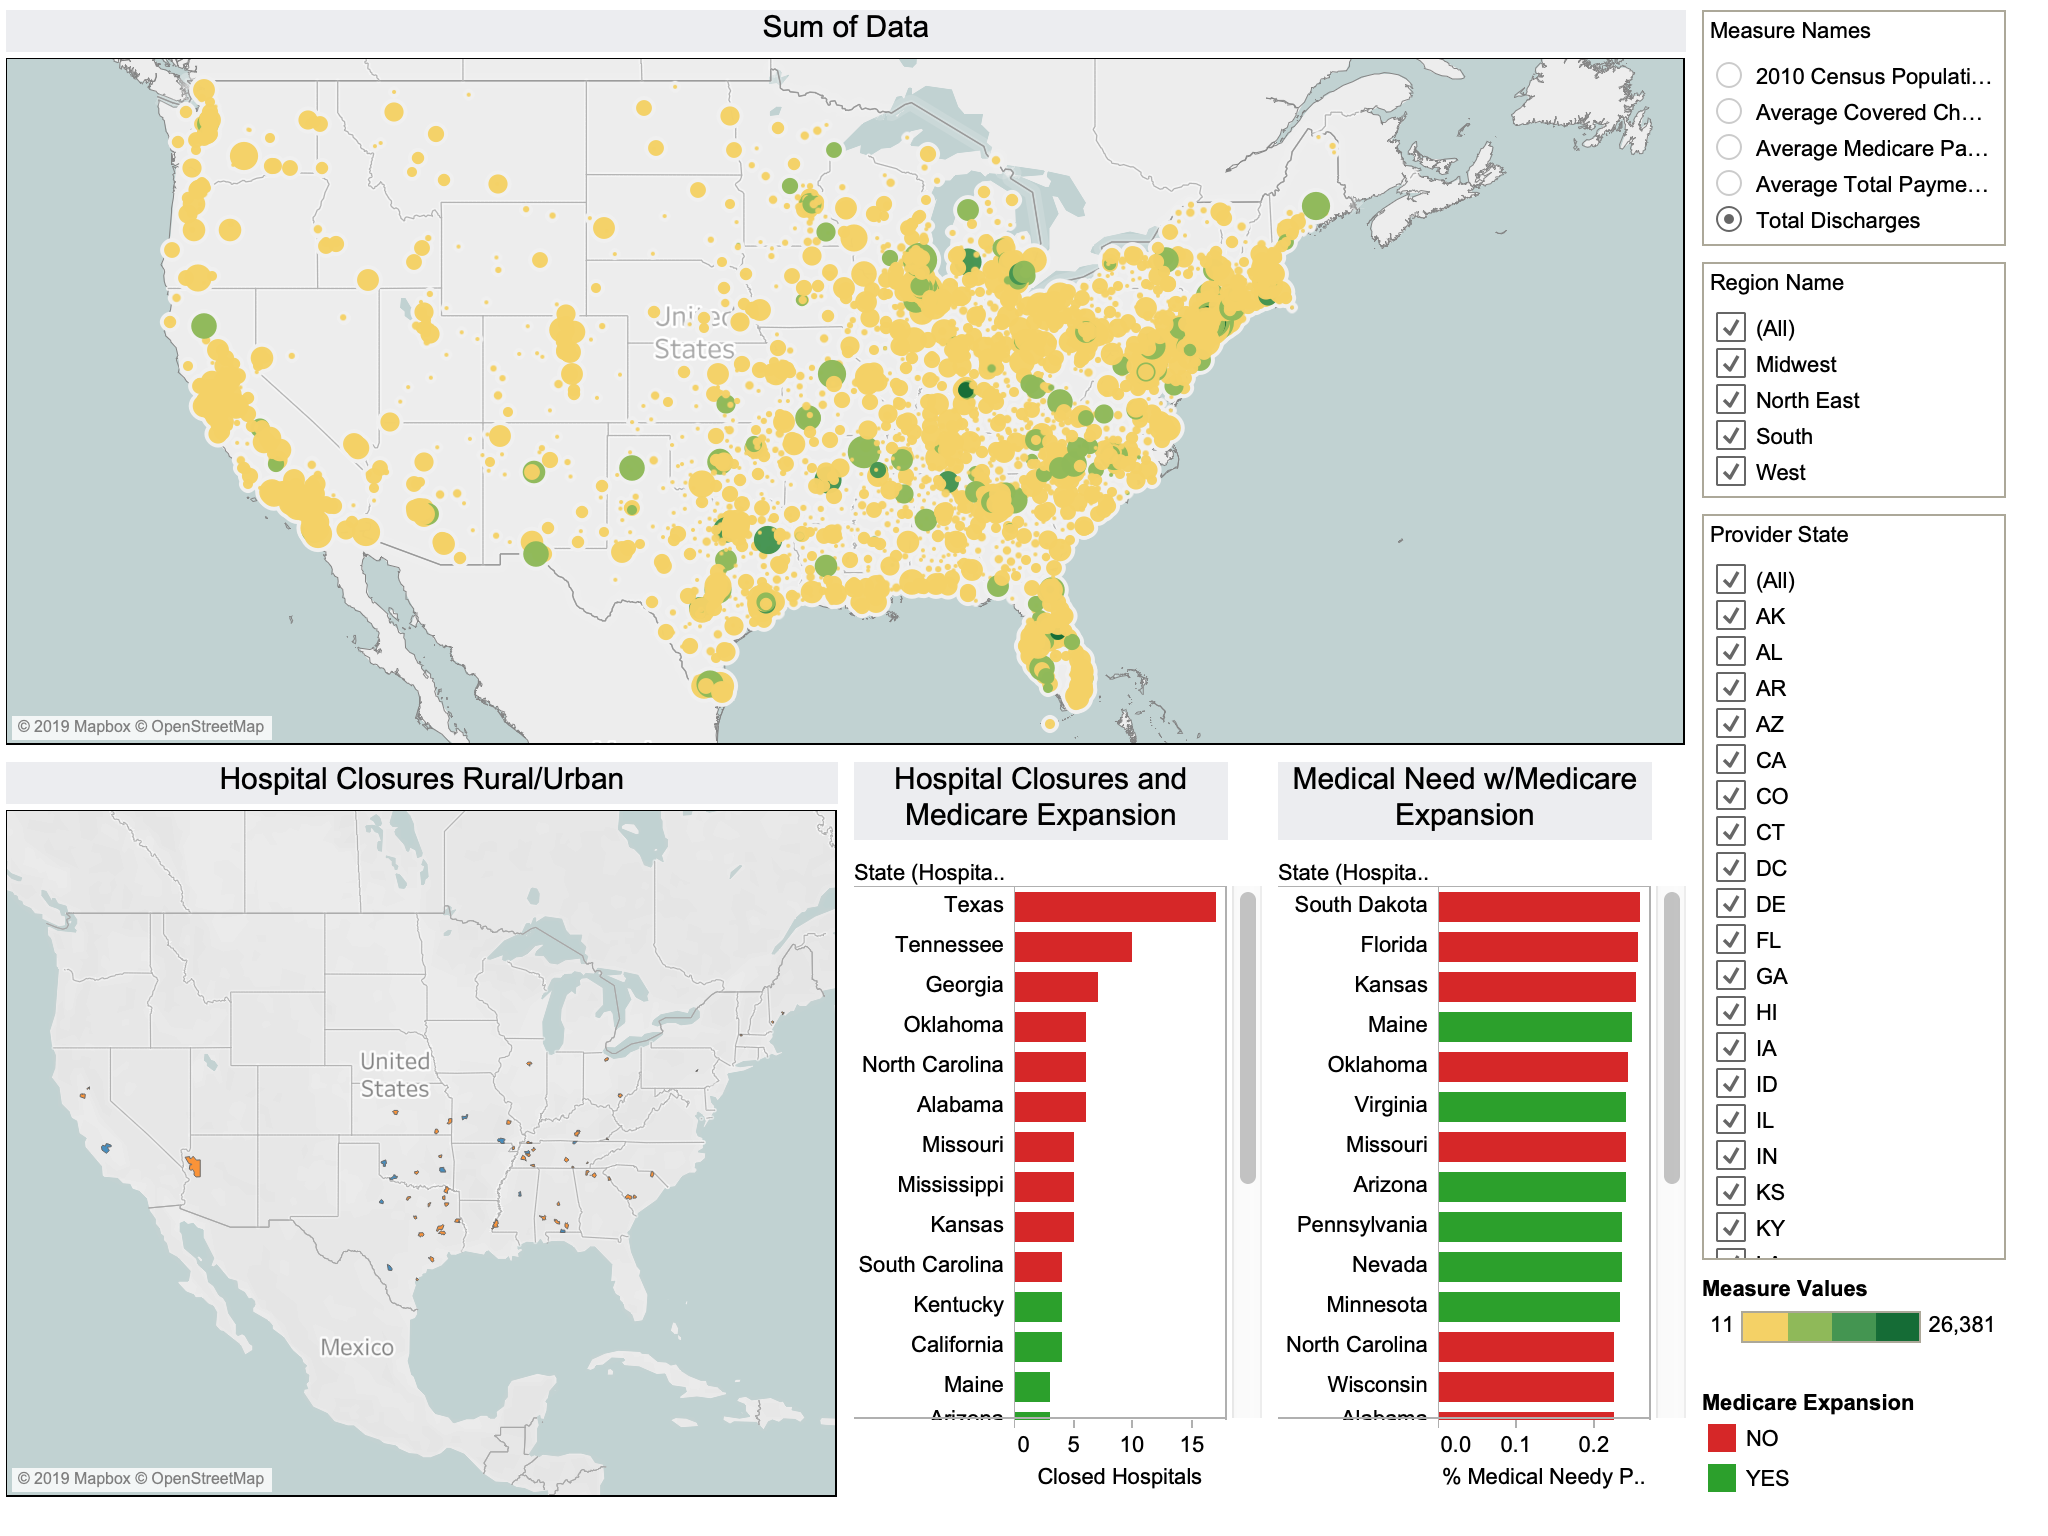
\includegraphics[width=0.4\textwidth]{Dashboard.png}
\caption{\emph{Tableau} Dashboard.}
\label{dashboard} 
\end{center}
\end{figure}
The resulting graphics are highly interactive and allows the user to select and display highly detailed information. As shown in figure \ref{Texas_Figure}, the user can display information by state as well as include text labels in the graphic. This graphic shows the average medicare payments made withing the counties that had at least one hospital closure.

\begin{figure}[htbp]
\begin{center}
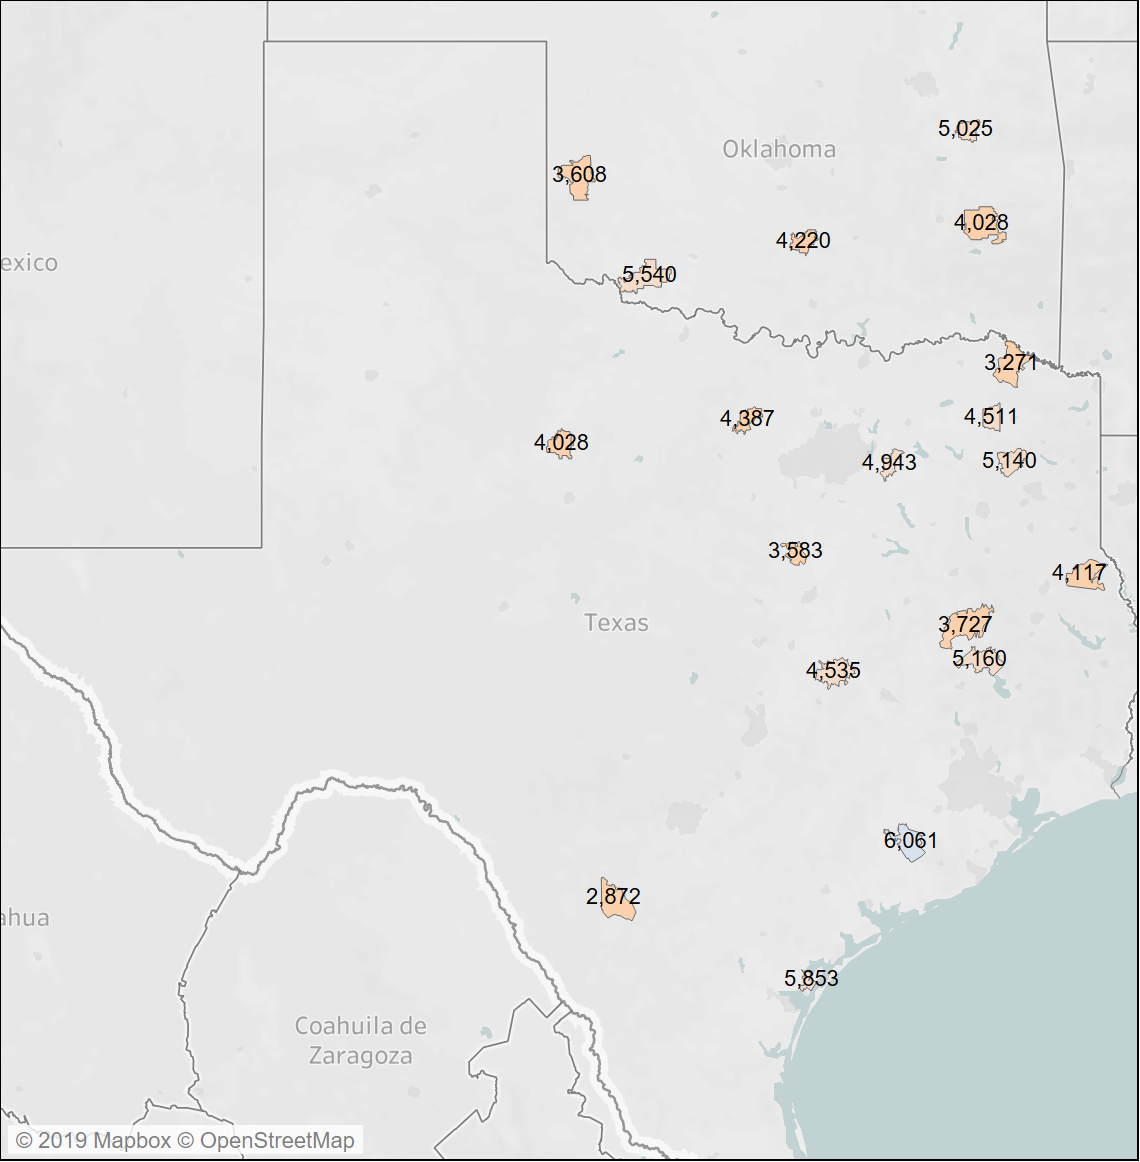
\includegraphics[width=0.4\textwidth]{MEDIAN_MED_PMT.png}
\caption{Median Medicare Payments in Texas.}
\label{Texas_Figure} 
\end{center}
\end{figure}

Null values were excluded from the overall analysis while geographical attributes like zip code, counties and states were rolled into geographic their respective hierarchies for easy drill down. 
\begin{table}[htbp]
\begin{center}
  \caption{Demographic information for states with at least one hospital closure}
    \begin{tabular}{|l|c|c|c|c|}
    \hline
    \multicolumn{1}{|c|}{State} & \multicolumn{1}{|c|}{Over 65} & \multicolumn{1}{|c|}{Under 19} & \multicolumn{1}{|c|}{Veteran} & \multicolumn{1}{|c|}{\# Closed Hospitals} \\
    \hhline{|=|=|=|=|=|}
    Texas & 15.07\% & 26.75\% & 6.93\% & 17.00 \\
    \hline
    Tennessee & 14.18\% & 23.45\% & 8.13\% & 10.00 \\
    \hline
    Georgia & 12.10\% & 26.60\% & 7.61\% & 7.00 \\
    \hline
    Oklahoma & 15.75\% & 24.44\% & 8.81\% & 6.00 \\
    \hline
    North Carolina & 14.41\% & 24.69\% & 8.34\% & 6.00 \\
    \hline
    Alabama & 14.14\% & 25.22\% & 8.53\% & 6.00 \\
    \hline
    Missouri & 15.89\% & 24.32\% & 8.27\% & 5.00 \\
    \hline
    Mississippi & 13.08\% & 27.00\% & 6.87\% & 5.00 \\
    \hline
    Kansas & 17.86\% & 24.52\% & 7.69\% & 5.00 \\
    \hline
    South Carolina & 13.18\% & 25.46\% & 9.20\% & 4.00 \\
    \hline
    Kentucky & 13.39\% & 24.32\% & 7.48\% & 4.00 \\
    \hline
    California & 12.60\% & 25.96\% & 5.24\% & 4.00 \\
    \hline
    Maine & 15.30\% & 22.00\% & 9.60\% & 3.00 \\
    \hline
    Arizona & 15.33\% & 28.15\% & 8.80\% & 3.00 \\
    \hline
    Virginia & 14.73\% & 23.48\% & 9.60\% & 2.00 \\
    \hline
    Pennsylvania & 16.18\% & 23.06\% & 7.59\% & 2.00 \\
    \hline
    Ohio  & 13.71\% & 25.12\% & 7.54\% & 2.00 \\
    \hline
    Minnesota & 16.30\% & 24.20\% & 7.15\% & 2.00 \\
    \hline
    Wisconsin & 15.30\% & 23.79\% & 7.39\% & 1.00 \\
    \hline
    South Dakota & 17.27\% & 25.88\% & 8.75\% & 1.00 \\
    \hline
    New York & 13.97\% & 24.06\% & 4.74\% & 1.00 \\
    \hline
    Nevada & 14.32\% & 24.97\% & 9.38\% & 1.00 \\
    \hline
    Michigan & 15.66\% & 23.95\% & 6.64\% & 1.00 \\
    \hline
    Massachusetts & 13.95\% & 22.93\% & 5.99\% & 1.00 \\
    \hline
    Illinois & 15.61\% & 24.21\% & 5.70\% & 1.00 \\
    \hline
    Florida & 17.01\% & 23.09\% & 8.82\% & 1.00 \\
    \hline
    \end{tabular}
     \label{tablel}
    \end{center}
\end{table}%

\section{Conclusion}

Hospital closures continue to grow within rural communities as various organizations and researchers decry the impact on the communities or what can be done to minimize these closures. These hospitals serve those in communities that are poorer, sicker and most elderly, which are referred here as high medical needs population. As shown in Figure \ref{HC_ME}, states that exhibited higher closure rates also have higher population percentages with Figure \ref{MN_ME} showing higher medical needed percentages in those states as well. Because majority of these higher medical needs patients and low income communities could only afford their access to medical service through Medicare insurance, the impact of states refusing the option provided under Affordable Care Act(ACA) to expand Medicare is seen as exacerbating both the hospitals’ financial challenges and the medical access challenges of these communities. It is also noted in this paper that most of the closures are in rural areas with 6 states with 5 or more rural hospital closures from 2010 to present.

\begin{figure}[htbp]
\centerline{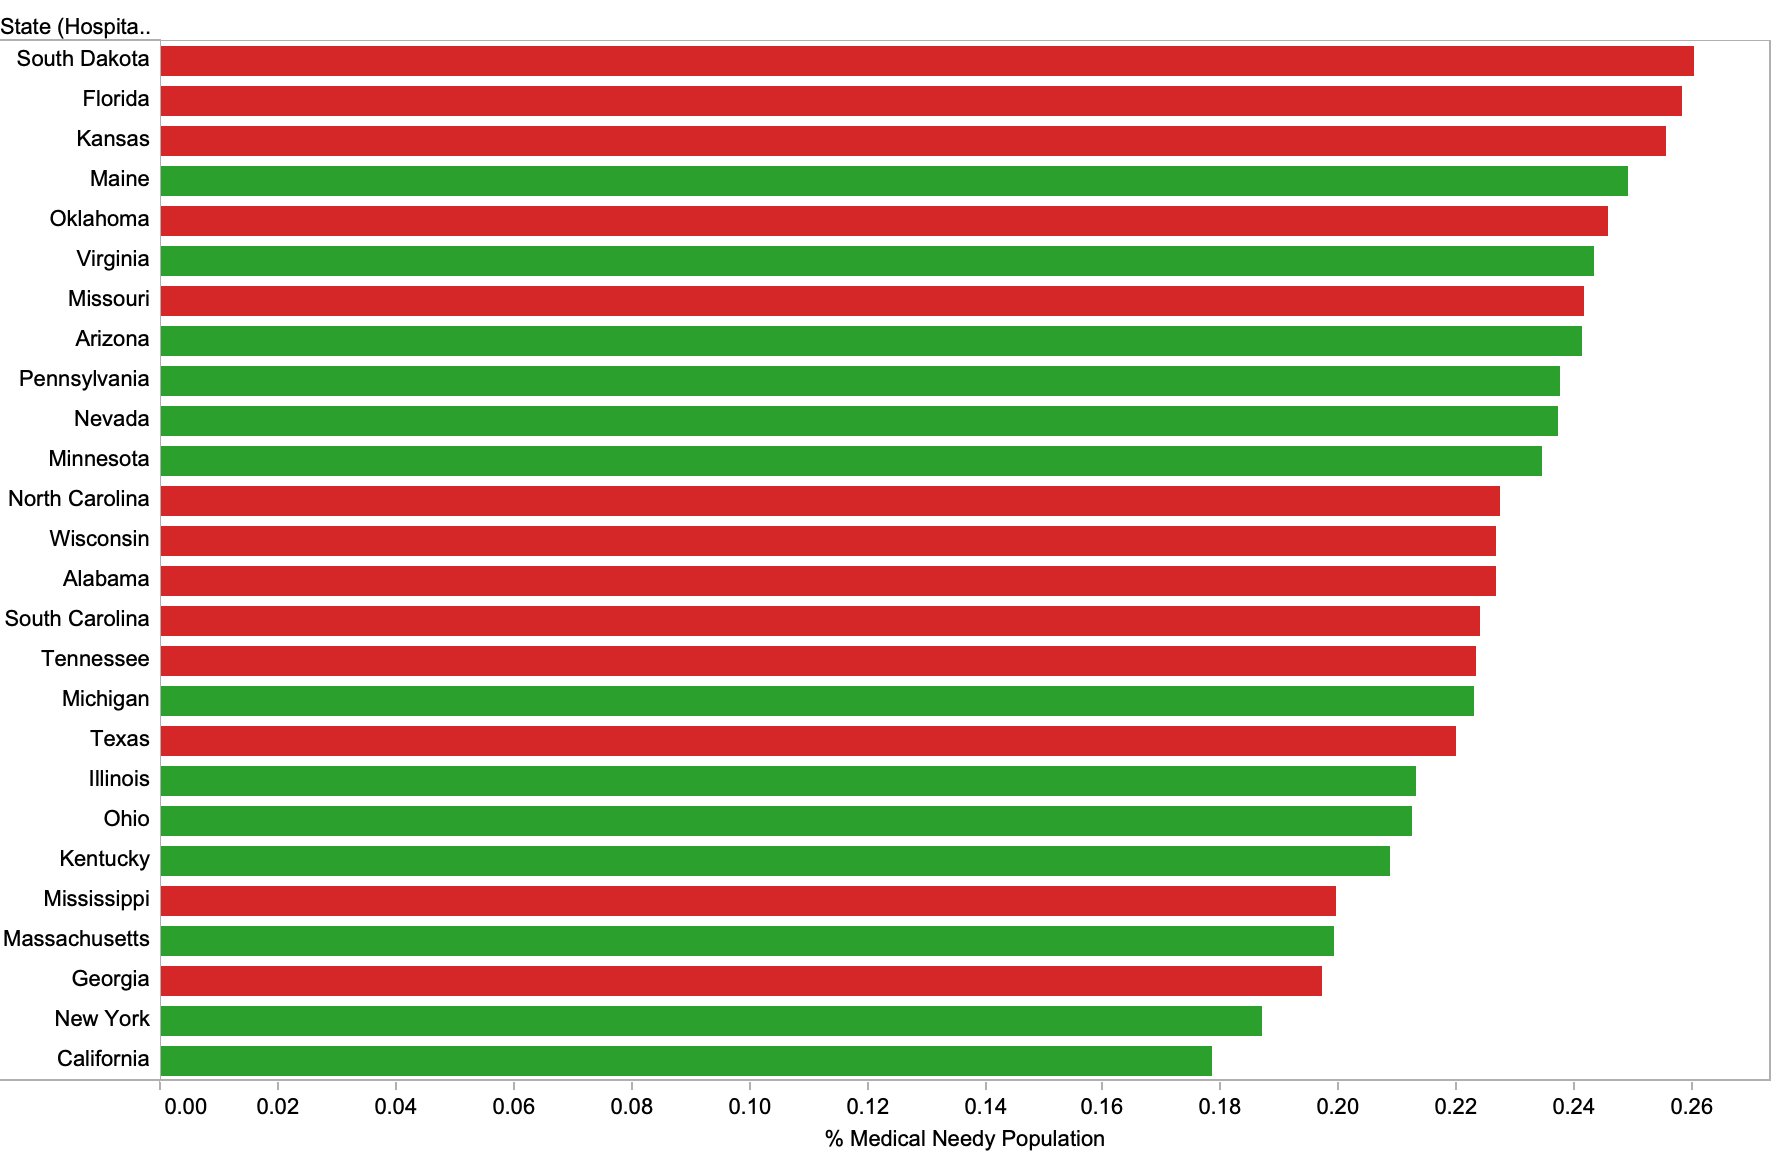
\includegraphics[width=0.5\textwidth]{MedicalNeedw_MedicareExpansion.png}}
\caption{Medical Need with Medicare Expansion(\textit{Red: No Green: Yes})}
\label{MN_ME}
\end{figure}
Many of those states are located in the south with all having a common characteristic—none have expanded Medicaid. Rural communities and small towns in non-expansion states have a greater percentage of uninsured residents with higher percentages of patients when they become seriously ill or injured. These closures have continued to cause an adverse effect on the areas they serve. There will need to be additional research to detail the effects of non-Medicaid expansion and what can be done for residents in these areas who fall victim to these closures \cite{searing}.

\section{Future Work}
This research has mostly focused on the visualization aspect to explore the relationship of population, Medicare payments, hospital closure, etc. This initial visual look has allowed us to have a reason to believe that states that are refusing Medicare expansion could help their higher medical needs communities better and reduce hospital closures by reversing this devastating policy position. We however recognize the limitations of this analysis and recommend future work to use larger volumes of data to explore these correlation assertions we are making. Additional research work could be done to explore other ways of keeping the hospitals open other than Medicaid expansion with the caveat that the demographics in question is lower income and requires assistance. We have also explored the idea that rural areas are have higher medical needs and high hospital closures. Further analysis could look at local policies that can help mitigate this challenge. It is also important to look at the impact of hospital closures, non-Medicare expansions on other socioeconomic factors like employment, median income, productivity and neighborhood out migrations.

\section{GitHub}
For access to the project data, \emph{MS Excel}, \emph{Tableau}, and image files please go to the following GitHUb location:
\hyperlink{https://github.com/laciotti/dsc611_Final_Project}{DSC-611 Group A Repository} or visit the following url: \url{https://github.com/laciotti/dsc611_Final_Project}


\section*{Acknowledgment}

We would also like to show our gratitude to the DSC-611 class for sharing their thought throughout the course, and we thank Dr. Alexander Hohl for his continued support through out the semester. We would also like to thank the developers of \LaTeX which was utilized to typeset this document. Without it, the formatting and sizing of items would have proven to troublesome at best.



\nocite{*}
\bibliographystyle{IEEEtran} % We choose the "plain" reference style
\bibliography{refs} % Entries are in the "refs.bib" file

\end{document}
